% This is part of Un soupçon de mathématique sans être agressif pour autant
% Copyright (c) 2012
%   Laurent Claessens
% See the file fdl-1.3.txt for copying conditions.

% This is part of Un soupçon de mathématique sans être agressif pour autant
% Copyright (c) 2012-2014
%   Laurent Claessens
% See the file fdl-1.3.txt for copying conditions.


\usepackage{etex}
\usepackage{ifthen}
%\usepackage{pdfsync}       % This package is obsolete : compile with pdflatex -synctex=1 instead.

\usepackage{latexsym}
\usepackage{amsfonts}
\usepackage{amsmath}
\usepackage{amsthm}
\usepackage{amssymb}
\usepackage{bbm}
\usepackage{mathrsfs}           
\usepackage{mathabx}           % Pour \divides

\usepackage{framed} % pour oframed
\usepackage{wrapfig}

\usepackage{calc}   % Les dépendances de phystricks si on n'utilise que le pdf.
%\usepackage{pstricks,pst-eucl,pstricks-add,calc,pst-math}   % Les dépendances de phystricks. Peut être qu'il faut ajouter catchfile


% Les dépendances de phystricks en mode Tikz
\usepackage{tikz}
\usepackage{calc}
\usetikzlibrary{calc}
\usetikzlibrary{patterns}

\usetikzlibrary{external}
\tikzexternalize
%\newcommand{\tikzsetnextfilename}[1]{}
\newcounter{defHatch}
\newcounter{defPattern}
\setcounter{defHatch}{0}
\setcounter{defPattern}{0}


\usepackage{graphicx}                   % Pour l'inclusion d'image en pfd.

%\newcommand{\EpsOrPdfincludegraphics}[2][]{%
%        \ifpdf
%            \includegraphics[#1]{#2.png}
%        \else
%            \includegraphics[#1]{#2.eps}
%        \fi
%        }

\usepackage{subfigure}

\usepackage{fancyvrb}
\usepackage{stmaryrd}       % Pour le \obslash
\usepackage{xstring}        % Utilisé pour les références vers wikipédia
\usepackage{cases}
\usepackage{lscape}         % pour l'environnement landscape, utilisé dans la correction corr0076.tex
\usepackage{multicol}
\setlength{\columnseprule}{0.5pt}
\usepackage{import}         % Pour le hack qui sert à inclure GeomAnal

% TODO : n'en utiliser qu'un
\usepackage[normalem]{ulem}     % Pour le barré, commande \sout
\usepackage{soul}       % Pour le barré, commande \st

\usepackage[all]{xy}

\let\second\undefined      % le paquet amthabx définit \second
\let\degree\undefined       % le paquet amthabx définit \degree
%\usepackage[cdot,thinqspace,amssymb]{SIunits} 
\usepackage[parse-numbers=false,binary-units=true,detect-all=true,per-mode=symbol]{siunitx} 
\newcommand{\unit}[2]{\SI{#1}{#2}}
 % L'option amssymb sert à éviter un conflit avec la commande \square de amssymb. Note qu'elle n'est plus accessible. Si tu en as besoin, faudra RTFM
%ftp://ftp.belnet.be/packages/ctan/macros/latex/contrib/SIunits/SIunits.pdf

\usepackage[nottoc]{tocbibind}
\usepackage[numbers]{natbib}

%%%%%%%%%%%%%%%%%%%%%%%%%%
%
%   Trucs mathématiques
%
%%%%%%%%%%%%%%%%%%%%%%%%

% ENSEMBLES DE NOMBRES
\newcommand{\eA}{\mathbbm{A}}
\newcommand{\eC}{\mathbbm{C}}
\newcommand{\eD}{\mathbbm{D}}
\newcommand{\eE}{\mathbbm{E}}
\newcommand{\eF}{\mathbbm{F}}
\newcommand{\eG}{\mathbbm{G}}
\newcommand{\eH}{\mathbbm{H}}
\newcommand{\eK}{\mathbbm{K}}
\newcommand{\eL}{\mathbbm{L}}
\newcommand{\eM}{\mathbbm{M}}
\newcommand{\eN}{\mathbbm{N}}
\newcommand{\eP}{\mathbbm{P}}
\newcommand{\eQ}{\mathbbm{Q}}
\newcommand{\eR}{\mathbbm{R}}
\newcommand{\eZ}{\mathbbm{Z}}

% ENSEMBLES de fonctions
\newcommand{\aL}{\mathcal{L}}       % Les applications linéaires
\newcommand{\aC}{\mathcal{C}}       % Les fonctions C^1, C^2 etc



\newcommand{\mF}{\mathcal{F}}
\newcommand{\mC}{\mathcal{C}}
\newcommand{\mG}{\mathcal{G}}
\newcommand{\mI}{\mathcal{I}}
\newcommand{\mL}{\mathcal{L}}
\newcommand{\mS}{\mathcal{S}}   % Utilisé pour l'espace des fonctions Schwartz
\newcommand{\mZ}{\mathcal{Z}}


\newcommand{\mtu}{\mathbbm{1}}              % La matrice unité

\DeclareMathOperator{\val}{val}     % valuation d'un polynôme
%\DeclareMathOperator{\opp}{opp}    % Les nombres négatifs


%\newcommand{\efrac}[2]{\frac{ \displaystyle #1 }{\displaystyle #2 }}
%%%%%%%%%%%%%%%%%%%%%%%%%%
%
%   Numérotations en tout genre
%
%%%%%%%%%%%%%%%%%%%%%%%%

\setcounter{tocdepth}{2}        % Profondeur de la table des matières
\setcounter{secnumdepth}{2}     % Profondeur dans le texte

\renewcommand{\thesubsection}{\thesection.\alph{subsection}}

%%%%%%%%%%%%%%%%%%%%%%%%%%
%
%   Les lignes magiques pour le texte en français.
%
%%%%%%%%%%%%%%%%%%%%%%%%

\usepackage[utf8]{inputenc}
\usepackage[T1]{fontenc}

\usepackage{listingsutf8}
%\lstset{language=python,basicstyle=\footnotesize,tabsize=3,numbers=left,numberstyle=\tiny,frame=single,commentstyle=\ttfamily\color[rgb]{0,0,0.5},stringstyle=\color[rgb]{0,0.5,0},title=\lstname,inputencoding=utf8/latin1}
\lstset{language=python,basicstyle=\footnotesize,tabsize=3,frame=single,commentstyle=\ttfamily\color[rgb]{0,0,0.5},stringstyle=\color[rgb]{0,0.5,0},title=\lstname,inputencoding=utf8/latin1}

\usepackage[fr]{exocorr}
\usepackage{textcomp}
\usepackage{lmodern}
\usepackage[a4paper,margin=2cm]{geometry} 
\usepackage[english,frenchb]{babel}


\usepackage{hyperref}                           %Doit être appelé en dernier.
\hypersetup{
colorlinks=true,
linkcolor=blue,
urlcolor=magenta,     % couleur des url
filecolor=magenta   % couleur des textes qui sont des liens
}

% Il me semble que cette commande doit être définie après l'appel à Babel.
\newcommand{\Ieme}{\up{\lowercase{ième}}\xspace}

%%%%%%%%%%%%%%%%%%%%%%%%%%
%
%   Les théorèmes et choses attenantes
%
%%%%%%%%%%%%%%%%%%%%%%%%


\newcounter{numtho}
\newcounter{numprob}

\makeatletter
\@addtoreset{numtho}{chapter}
%\@addtoreset{CountExercice}{chapter}
\@addtoreset{chapter}{part}
\makeatother

\newlength{\EnvSpace}
\setlength{\EnvSpace}{9pt}      % C'est la distance que je veux mettre avant et après les théorèmes, remarques, etc.

\newtheoremstyle{MyTheorems}%
        {\EnvSpace}{\EnvSpace}%
        {\itshape}%
        {}%
        {\bfseries}{.}%
        {\newline}%
        {}%
\newtheoremstyle{MyExamples}%
        {\EnvSpace}{\EnvSpace}%
        {}%
        {}%
        {\bfseries}{.}%
        {\newline}%
        {}%
\newtheoremstyle{MyRemarks}%
        {\EnvSpace}{\EnvSpace}%
        {}%
        {}%
        {\bfseries}{.}%
        {\newline}%
        {}%

%\theoremstyle{MyExamples}   %\newtheorem{exemple}[numtho]{Exemple}      % Pour unification, ne plus utiliser
%                            \newtheorem{example}[numtho]{Exemple}
\newcounter{CounterExample}
\renewcommand{\theCounterExample}{\thechapter.\arabic{CounterExample}}

% J'ai décidé de ne plus numéroter les choses encadrées. 8 avril 2014
\newenvironment{example}{\vspace{\EnvSpace}\refstepcounter{numtho}\noindent{\bf Exemple}\\\nopagebreak}{\phantom{a}\hfill $\triangle$\vspace{\EnvSpace}}
\newenvironment{Aretenir}{\refstepcounter{numtho}\begin{oframed}\noindent{\bf À retenir}\newline}{\end{oframed}\vspace{\EnvSpace}}
\newenvironment{Aprojeter}{\clearpage\phantom{a}\vfill}{\vfill\newpage}
\newenvironment{definition}[1][]{\refstepcounter{numtho}\begin{oframed}\noindent{\bf Définition}#1\newline}{\end{oframed}\vspace{\EnvSpace}}
\newenvironment{propriete}{\refstepcounter{numtho}\begin{oframed}\noindent{\bf Propriété}\newline}{\end{oframed}\vspace{\EnvSpace}}

\newenvironment{Enmini}{\begin{oframed}\noindent{\bf Mini résumé}\newline}{\end{oframed}\vspace{\EnvSpace}}
% Ce bout de code provient de BrunoJ
% https://brunoj.wordpress.com/2009/10/08/latex-the-framed-minipage/
\newsavebox{\fmbox}
 \newenvironment{fmpage}[1]
 {\begin{lrbox}{\fmbox}\begin{minipage}{#1}}
     {\end{minipage}\end{lrbox}
     \fbox{\usebox{\fmbox}}
 }

\theoremstyle{MyRemarks}    \newtheorem{remark}[numtho]{Remarque}

                \newtheorem{amusement}[numtho]{Amusement}
                \newtheorem{erreur}[numtho]{Error}
                \newtheorem{probleme}[numprob]{\fbox{\bf Problèmes et choses à faire}}


\theoremstyle{MyTheorems}
\newtheorem{lemma}[numtho]{Lemme}
\newtheorem{corollary}[numtho]{Corollaire}
\newtheorem{theorem}[numtho]{Théorème}      
\newtheorem{proposition}[numtho]{Proposition}      


\renewcommand{\thenumtho}{\thechapter.\arabic{numtho}}
% La numérotation des équations change dans les corrigés
\renewcommand{\theequation}{\thechapter.\arabic{equation}}
\renewcommand{\theCountExercice}{\arabic{CountExercice}}       % Ce compteur est défini dans SystemeCorr.sty
\newcommand{\defe}[2]{\textbf{#1}\index{#2}}

\renewcommand{\theenumi}{(\alph{enumi})}
\renewcommand{\theenumii}{(\alph{enumi}\arabic{enumii})}

\renewcommand{\labelenumi}{\theenumi}
\renewcommand{\labelenumii}{\theenumii}

\newcommand{\justification}{ {\small \begin{center}    Attention : vous devez laisser sur votre feuille les traces de vos recherches et les étapes intermédiaires de vos calculs !    \end{center}}}
    

    % L'une des deux est avec le nom et l'autre sans.
    \newenvironment{feuilleDS}[1]{\noindent Nom, Prénom : \begin{center}\large #1\\\justification\end{center}\setcounter{CountExercice}{0}  }{\clearpage}
    %\newenvironment{feuilleDS}[1]{\begin{center}\large #1\\\justification\end{center}\setcounter{CountExercice}{0}  }{\clearpage}


    \newenvironment{feuilleExo}[1]{\newpage\begin{center}\large #1\end{center}\setcounter{CountExercice}{0}  }{\clearpage}
    %\newenvironment{feuilleExo}[1]{\begin{center}\large #1\end{center}\setcounter{CountExercice}{0}  }{}

        
        \newcounter{numactivmentale}
        \setcounter{numactivmentale}{0}
        \newcounter{numExoMental}
        \setcounter{numExoMental}{0}
        \newenvironment{MentalActivity}{\setcounter{numExoMental}{0}\newpage\refstepcounter{numactivmentale}\section{Activité mentale \arabic{numactivmentale}}}{\newpage\hphantom{jj}\vfill\large C'est tout pour aujourd'hui\vfill\newpage}
        \newenvironment{mental}{\refstepcounter{numExoMental}\newpage\begin{center}\fbox{\huge Activité mentale \arabic{numactivmentale}}\\\huge Question \arabic{numExoMental}\end{center}\huge\vfill}{\vfill}


\newcommand{\enteteInterro}[3]{
    \begin{center}
        #1\\
        Intérogation #2, sujet #3
    \end{center}
    Nom, prénom, classe : \ldots\\
    \setcounter{CountExercice}{0}
}


%%%%%%%%%%%%%%%%%%%%%%%%%%
%
%   Les macros qui font des choses
%
%%%%%%%%%%%%%%%%%%%%%%%%

\newcommand{\mA}{\mathcal{A}}
\newcommand{\mO}{\mathcal{O}}
\newcommand{\mR}{\mathcal{R}}
\newcommand{\mT}{\mathcal{T}}
\newcommand{\mU}{\mathcal{U}}

\newcommand{\scal}[2]{ \langle #1,#2\rangle }

\newcommand{\tq}{\text{ tel que }}
\newcommand{\tqs}{\text{ tels que }}
\newcommand{\quext}[1]{ \footnote{\textsf{#1}}  }
\newcommand{\info}[1]{\texttt{#1}}
\newcommand{\vect}[1]{\overrightarrow{#1}}    % Cette macro est codée en dur dans phystricksDefVecteurAXDDGP et dans d'autres

\newcommand{\VarAbs}{\text{Var}_{\text{abs}}}
\newcommand{\VarRel}{\text{Var}_{\text{rel}}}

\newcommand{\normal}{\lhd}
\newcommand{\swS}{\mathscr{S}}          % L'ensemble des fonctions Schwartz

%\newcommand{\defD}{\mathscr{D}}     % Ensemble de définition d'une fonction
\newcommand{\defD}{D}                % Le D avec des croles était impossible à comprendre pour les élèves.

\newcommand{\Borelien}{\mathcal{B}\text{or}}       % Les boréliens
\newcommand{\tribA}{\mathcal{A}}            % Une tribu A
\newcommand{\tribB}{\mathcal{B}}            
\newcommand{\tribF}{\mathcal{F}}            % Une tribu F

\newcommand{\affE}{\mathcal{E}}            % Un espace affine E
\newcommand{\affF}{\mathcal{F}}            
\newcommand{\affG}{\mathcal{G}}            

\newcommand{\statS}{\mathcal{S}}            % Un modèle statistique
\newcommand{\partP}{\mathcal{P}}            % L'ensemble des parties d'un ensemble

\newcommand{\polyP}{\mathcal{P}}            % L'ensemble des polynômes

\newcommand{\dB}{\mathscr{B}}       % la distribution de Bernoulli
\newcommand{\dE}{\mathscr{E}}       % la distribution exponentielle
\newcommand{\dG}{\mathscr{G}}       % la distribution géométrique.
\newcommand{\dM}{\mathscr{M}}       % la distribution multinomiale
\newcommand{\dN}{\mathscr{N}}       % la distribution normale.
\newcommand{\dP}{\mathscr{P}}       % la distribution de Poisson.
\newcommand{\dT}{\mathscr{T}}       % la distribution de Student
\newcommand{\dU}{\mathscr{U}}       % la distribution uniforme

\newcommand{\hL}{\mathscr{L}}       
\newcommand{\cL}{\hL}           % Pour la partie Chafai

\newcommand{\modE}{\mathcal{E}}         % Le E des modules
\newcommand{\modF}{\mathcal{F}}         % Le F des modules
\newcommand{\hH}{\mathscr{H}}           % Le H des espaces de Hilbert

%%%%%%%%%%%%%%%%%%%%%%%%%%
%
%   Bibliographie, index et liste des notations
%
%%%%%%%%%%%%%%%%%%%%%%%%

\usepackage{makeidx}
\usepackage[nottoc]{tocbibind}      % Le paquetage qui fait en sorte que la biblio soit inclue correctement dans la table des matières.
\usepackage[refpage]{nomencl}
\renewcommand{\nomname}{Liste des notations}
%
%   Comment introduire des éléments dans l'index des notations.
%
% La liste des tags à mettre pour bien classer mes notations est :
% T     pour la topologie et théorie des ensembles
%
% La syntaxe est facile, par exemple 
%       $\SL(2,\eR)$\nomenclature[G]{$\SL(2,\eR)$}{Le groupe de matrices deux par deux de déterminant 1.}
%\renewcommand{\nomgroup}[1]{%
%    \ifthenelse{\equal{#1}{A}}{\item[\textbf{Algèbre}]}{}%
%    \ifthenelse{\equal{#1}{G}}{\item[\textbf{Géométrie}]}{}%
%    \ifthenelse{\equal{#1}{R}}{\item[\textbf{Théorie des groupes}]}{}%
%    \ifthenelse{\equal{#1}{P}}{\item[\textbf{Probabilités et statistique}]}{}%
%    \ifthenelse{\equal{#1}{Y}}{\item[\textbf{Analyse}]}{}%
%    \ifthenelse{\equal{#1}{M}}{\item[\textbf{Chaînes de Markov}]}{}%
%}

%%%%%%%%%%%%%%%%%%%%%%%%%%
%
%   DeclareMathOperator
%
%%%%%%%%%%%%%%%%%%%%%%%%

\DeclareMathOperator{\signe}{sgn}
\DeclareMathOperator{\Vol}{Vol}
\DeclareMathOperator{\Int}{Int}     % Intérieur d'un ensemble.
\DeclareMathOperator{\Ind}{Ind}     % l'indice d'un chemin en analyse complexe
\DeclareMathOperator{\Diam}{Diam}   
\DeclareMathOperator{\id}{Id}   
\DeclareMathOperator{\Graph}{Graph} 
\DeclareMathOperator{\pr}{\texttt{proj}}
\DeclareMathOperator{\dom}{dom}

\DeclareMathOperator{\Graphe}{Gr}
\DeclareMathOperator{\Spec}{Spec}   % spectre d'un opérateur
\DeclareMathOperator{\arctg}{arctg}
\DeclareMathOperator{\cotg}{cotg}
\DeclareMathOperator{\cosec}{cosec}
\DeclareMathOperator{\arcsinh}{arcsinh}

\DeclareMathOperator{\GL}{GL}   % le groupe linéaire
\DeclareMathOperator{\PGL}{PGL}   % le groupe projectif
\DeclareMathOperator{\SO}{SO}           
\DeclareMathOperator{\SL}{SL}           
\DeclareMathOperator{\PSL}{PSL}   % Le groupe modulaire SL(2,Z)/Z2
\DeclareMathOperator{\gO}{O}           
\DeclareMathOperator{\SU}{SU}           
\DeclareMathOperator{\gU}{U}           

\DeclareMathOperator{\Reel}{Re}        % La partie réelle d'un nombre complexe

\DeclareMathOperator{\Image}{Image}        % ... avec \Image qui donne l'image d'une fonction ou d'un opérateur.
\DeclareMathOperator{\rang}{rg}   
\DeclareMathOperator{\Kernel}{Ker}
\DeclareMathOperator{\Domaine}{Dom}
\DeclareMathOperator{\Span}{Span}
\DeclareMathOperator{\Hom}{Hom}
\DeclareMathOperator{\End}{End}     % L'ensemble des endomorphismes
\DeclareMathOperator{\tr}{Tr}       % la trace
\DeclareMathOperator{\Majorant}{Maj}
\DeclareMathOperator{\codim}{codim} % pour la codimension.
\DeclareMathOperator{\diam}{diam} % le diamètre d'un ensemble.

\DeclareMathOperator{\Var}{Var}     % Variance d'une variable aléatoire.
\DeclareMathOperator{\Fun}{\texttt{Fun}}     % Ensemble des applications d'un ensemble vers l'autre.
\DeclareMathOperator{\Cov}{Cov}     % la covariance.
\DeclareMathOperator{\gr}{gr}     % le groupe engendré
\DeclareMathOperator{\pgcd}{pgcd}     
\DeclareMathOperator{\ppcm}{ppcm}     
\DeclareMathOperator{\Frob}{Frob}     
\DeclareMathOperator{\Card}{Card}       % Le cardinal d'un ensemble.
\DeclareMathOperator{\Stab}{Stab}       % Le stabilisateur d'un point sous l'action d'un groupe.

\DeclareMathOperator{\Frac}{Frac}       % le corps des fractions d'un anneau
\DeclareMathOperator{\Aff}{Aff}         %  l'espace affine engendré

\newenvironment{subproof}{\begin{description}}{\end{description}}

\newcommand{\telque}{\vert\,}
\newcommand{\donc}{\Rightarrow}

\usepackage{mathtools}
\mathtoolsset{showonlyrefs}



\makeindex
\makenomenclature

\begin{document}

\corrPosition{1}


% This is part of Un soupçon de mathématique sans être agressif pour autant
% Copyright (c) 2012
%   Laurent Claessens
% See the file fdl-1.3.txt for copying conditions.

\thispagestyle{empty}
\begin{center}
  \begin{minipage}{15cm}
    \hrule\par
    \vspace{2mm}
    \begin{center}
    \Huge \bfseries Un soupçon de mathématiques sans être agressif pour autant \par
    \end{center}
    \hrule\par
  \end{minipage}
\end{center}

\vspace{2cm}

\begin{center}
    Laurent \textsc{Claessens}\\
    \today\\
    Dernière version :\\
    \url{http://student.ulb.ac.be/~lclaesse/smath.pdf}
\end{center}

\vfill

\begin{center}

           \ifpdf
            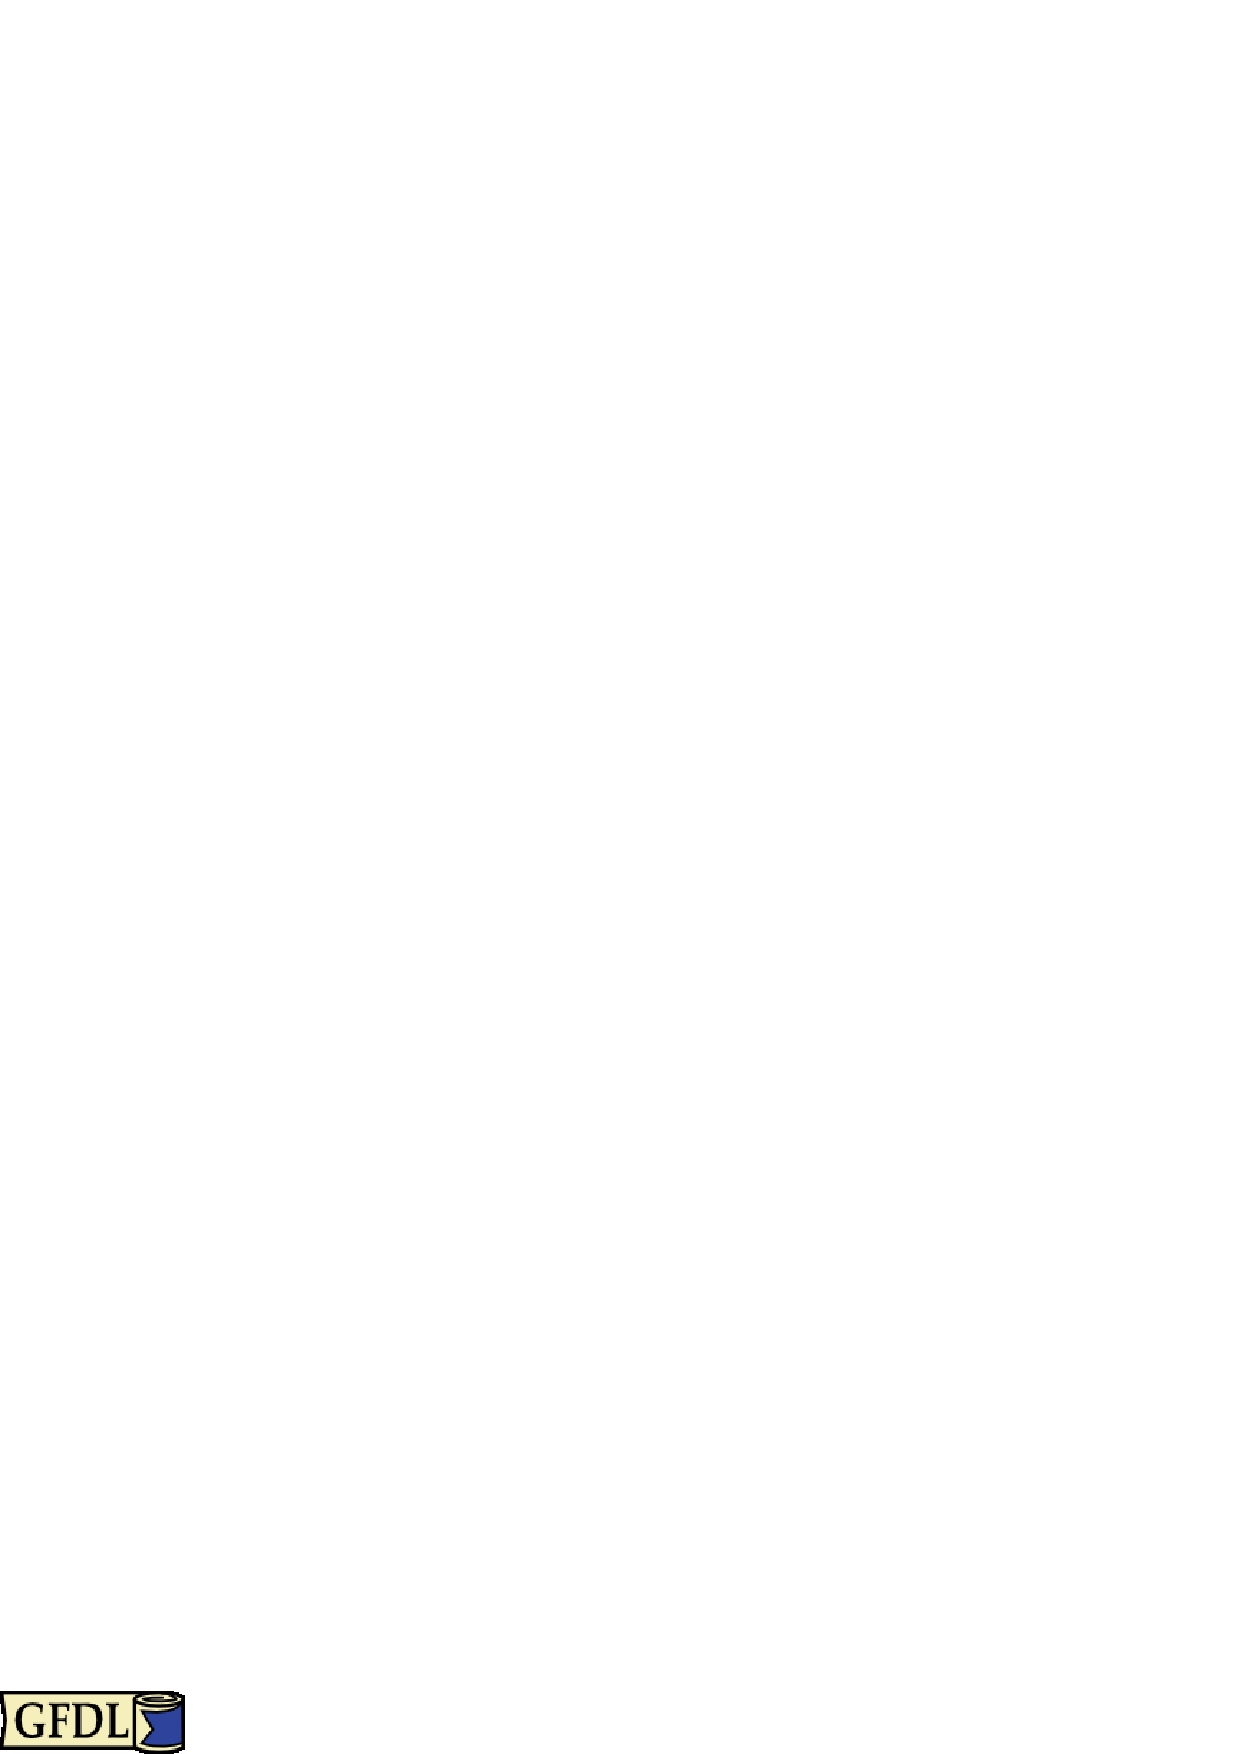
\includegraphics[width=1cm]{gfdl-logo-small.png}
        \else
            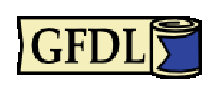
\includegraphics[width=1cm]{gfdl-logo-small.eps}
        \fi

Copyright (c) 2012  Laurent Claessens

Permission is granted to copy, distribute and/or modify this document under the terms of the \href{http://www.gnu.org/licenses/fdl-1.3.html}{GNU Free Documentation License}, Version 1.3 or any later version published by the Free Software Foundation; with no Invariant Sections, no Front-Cover Texts, and no Back-Cover Texts. A copy of the license is included in the chapter entitled ``GNU Free Documentation~License''.

\vspace{0.5cm}

Vous avez le droit de copier, distribuer et modifier ce document pourvu que vous suiviez les règles de la \wikipedia{fr}{GFDL}{GNU Free Documentation License}. Vous trouverez les sources \LaTeX\ sur gitorious :\\
    \url{https://www.gitorious.org/smath/smath/trees/master}

\end{center}


\tableofcontents

\newpage

\part{Seconde}
% This is part of Un soupçon de mathématique sans être agressif pour autant
% Copyright (c) 2012
%   Laurent Claessens
% See the file fdl-1.3.txt for copying conditions.

\chapter{Statistiques descriptives}

%+++++++++++++++++++++++++++++++++++++++++++++++++++++++++++++++++++++++++++++++++++++++++++++++++++++++++++++++++++++++++++
\section{Activité : mois de naissance}
%+++++++++++++++++++++++++++++++++++++++++++++++++++++++++++++++++++++++++++++++++++++++++++++++++++++++++++++++++++++++++++

Prendre les mois de naissance des élèves, en séparant les groupes.
\begin{enumerate}
    \item
        Quel groupe a la proportion de naissance en mars la plus grande ?
    \item
        En tout quelle est la proportion des naissances en avril ?
    \item 
        Est-ce qu'on peut voir l'effet comme quoi les mois de \( 31\) jours son plus longs ? 
        \begin{enumerate}
            \item
                Quelle est la proportion d'élèves nés dans un mois de \( 31\) jours ?
            \item
                Il y a \( 7\) mois de $31$ jours contre \( 5\) de moins. Donc le résultat est biaisé.
            \item
                Calculer la \emph{fréquence} des naissances en naissances par mois.
        \end{enumerate}
\end{enumerate}

%+++++++++++++++++++++++++++++++++++++++++++++++++++++++++++++++++++++++++++++++++++++++++++++++++++++++++++++++++++++++++++
\section{Regardons des graphiques}
%+++++++++++++++++++++++++++++++++++++++++++++++++++++++++++++++++++++++++++++++++++++++++++++++++++++++++++++++++++++++++++

Les graphiques sont souvent tirés de wikipédia. Si vous voulez plus d'informations, lisez \url{http://www.manicore.com/}, ou bien regardez le cours \href{http://www.mines-paristech.fr/ingenieurcivil/SitesIC/Balado/Climat_som.html}{en ligne}, en particulier la deuxième heure du troisième cours donne les facteurs d'émissions dans le monde et en France.

%---------------------------------------------------------------------------------------------------------------------------
\subsection{Émissions par secteurs}
%---------------------------------------------------------------------------------------------------------------------------

\includegraphics[width=17cm]{Emission_de_GES.png}
Graphique en provenance de l'article \wikipedia{fr}{Gaz_à_effet_de_serre}{gaz à effet de serre} de wikipédia.

\begin{enumerate}
    \item
        Quel est le secteur qui émets le plus ?
    \item
        Est-ce que l'agriculture émet beaucoup de dioxyde de carbone ?
    \item
        À partir des deux graphiques du bas, est-ce que vous êtes capables de retrouver le \( 12.5\%\) de l'agriculture donnés dans le graphique du haut ?
\end{enumerate}

%---------------------------------------------------------------------------------------------------------------------------
\subsection{Découvertes de pétrole}
%---------------------------------------------------------------------------------------------------------------------------

Regardons un instant le graphique suivant, provenant de l'article \wikipedia{fr}{Pic_pétrolier}{Pic pétrolier} de wikipédia.

\includegraphics[width=17cm]{Decouvertes-petrole.png}

\begin{enumerate}
    \item
        Quelle est l'année où on a découvert le plus de pétrole ?
    \item
        Quelle est l'année où on a consommé le plus de pétrole ?
    \item
        En quelles années on a consommé autant qu'on a découvert ?
    \item
        Que pensez-vous de l'affirmation «ce qui reste comme réserve est la surface jaune au-dessus de la ligne rouge» ?
\end{enumerate}
Pour aller plus loin, remarquer la cassure assez nette de la croissance de la production vers 1975. Juste par curiosité, faites quelque recherches sur l'histoire de la croissance économique, de la dette publique et le chômage en France (et en Europe). Est-ce que les années 1970 ont été spéciales de ce point de vue ?

%---------------------------------------------------------------------------------------------------------------------------
\subsection{Températures}
%---------------------------------------------------------------------------------------------------------------------------

\includegraphics[width=17cm]{Instrumental_Temperature_Record_fr.png}
Graphique en provenance de l'article \wikipedia{fr}{Réchauffement_climatique}{réchauffement climatique} de wikipédia.

Le zéro de ce graphique est la moyenne 1961-1990.

\begin{enumerate}
    \item
        Quelle est la dernière année «normale» ?
    \item
        Quelle est l'année la plus chaude ?
    \item
        Quelle est l'année la plus froide ?
\end{enumerate}

%---------------------------------------------------------------------------------------------------------------------------
\subsection{Consommation de pétrole}
%---------------------------------------------------------------------------------------------------------------------------

Lire le tableau suivant :
\begin{center}
\begin{tabular}[h]{|c|c|c|c|c|c|c|c|c|}
année&
2001&
2002&
2003&
2004&
2005&
2006&
2007&
2008\\
consommation (Mb/j)&
76,8&
77,7&
79,1&
81,8&
83,1&
83,8&
84,9&
84,5
\end{tabular}
\end{center}

Calculer le pourcentage d'augmentation année par année. Que s'est-il passé en 2008 ?

%---------------------------------------------------------------------------------------------------------------------------
\subsection{À faire fonctionner}
%---------------------------------------------------------------------------------------------------------------------------

Les graphiques montrent
\begin{enumerate}
    \item

        À la figure \ref{LabelFigautomaticDSpcb}, \( y=\) proportion des étudiants ayant obtenu plus que \( x\)
    \item
        À la figure \ref{LabelFigautomaticDSpbt}, \( y=\) moyenne des étudiants ayant obtenu plus que \( x\). Par construction, le tout premier point de ce graphique est la moyenne de tout le groupe.
    \item
        À la figure \ref{LabelFigautomaticDSavb}, \( y=\) proportion des étudiants ayant obtenu dans \( \mathopen[ x-0.5 , x+0.5 \mathclose]\).
\end{enumerate}

\newcommand{\CaptionFigautomaticDSpcb}{Moyenne des étudiants ayant obtenus plus que \( x\)}
\input{Fig_automaticDSpcb.pstricks}

\newcommand{\CaptionFigautomaticDSpbt}{Proportion des étudiants ayant obtenus plus que \( x\)}
\input{Fig_automaticDSpbt.pstricks}

\newcommand{\CaptionFigautomaticDSavb}{proportion des étudiants ayant obtenu dans \( x\pm 0.5\)}
\input{Fig_automaticDSavb.pstricks}

%+++++++++++++++++++++++++++++++++++++++++++++++++++++++++++++++++++++++++++++++++++++++++++++++++++++++++++++++++++++++++++
\section{Théorie}
%+++++++++++++++++++++++++++++++++++++++++++++++++++++++++++++++++++++++++++++++++++++++++++++++++++++++++++++++++++++++++++

\begin{definition}
    Une \defe{population}{population} est un ensemble fini. Une \defe{série statistique}{série statistique} sur une population est une fonction qui à chaque élément (individu) de la population fait correspondre une valeur.

    L'\defe{effectif}{effectif} d'une valeur est le nombre d'individus correspondant à la valeur.

    La \defe{fréquence}{fréquence} d'une valeur est le rapport
    \begin{equation}
        f=\frac{ \text{effectif de la valeur} }{ \text{effectif total} }
    \end{equation}
    où par «effectif total» nous entendons la taille de la population totale.
\end{definition}



\chapter{Exercices}

%+++++++++++++++++++++++++++++++++++++++++++++++++++++++++++++++++++++++++++++++++++++++++++++++++++++++++++++++++++++++++++
\section{Repères, distances, milieu}
%+++++++++++++++++++++++++++++++++++++++++++++++++++++++++++++++++++++++++++++++++++++++++++++++++++++++++++++++++++++++++++

\Exo{Seconde-0001}
\Exo{Seconde-0002}
\Exo{Seconde-0003}
\Exo{Seconde-0004}
\Exo{Seconde-0005}
\Exo{Seconde-0006}
\Exo{Seconde-0007}
\Exo{Seconde-0008}
\Exo{Seconde-0009}
\Exo{Seconde-0010}
\Exo{Seconde-0011}
\Exo{Seconde-0012}
\Exo{Seconde-0013}

%+++++++++++++++++++++++++++++++++++++++++++++++++++++++++++++++++++++++++++++++++++++++++++++++++++++++++++++++++++++++++++
\section{Petits exercices de calcul mental}
%+++++++++++++++++++++++++++++++++++++++++++++++++++++++++++++++++++++++++++++++++++++++++++++++++++++++++++++++++++++++++++

\Exo{Seconde-0014}
\Exo{Seconde-0015}
\Exo{Seconde-0016}
\Exo{Seconde-0017}
\Exo{Seconde-0018}
\Exo{Seconde-0019}
\Exo{Seconde-0020}


\part{Première STG}
% This is part of Un soupçon de mathématique sans être agressif pour autant
% Copyright (c) 2012
%   Laurent Claessens
% See the file fdl-1.3.txt for copying conditions.

\chapter{Proportions}

Nous disons qu'un gaz est en concentration de une \defe{partie par million}{partie par million} si un million de grammes d'air contient un gramme du gaz. Voici quelque chiffre concernant l'évolution de la concentration de \( CO_2\) dans l'atmosphère; les chiffres sont en \( \unit{}{ppm}\) :
\begin{center}
\begin{tabular}{|c|c|c|}
    \hline
    1750    &   2005    &   1012\\
    \hline
    280&380&395\\
    \hline
\end{tabular}
\end{center}
Pour information, cette concentration n'a pas dépassé les \unit{300}{ppm} depuis au moins \( 600.000\) ans.



\Exo{Premiere-0001}
\Exo{Premiere-0002}
\Exo{Premiere-0003}
\Exo{Premiere-0004}
\Exo{Premiere-0005}
\Exo{Premiere-0006}
\Exo{Premiere-0007}
\Exo{Premiere-0008}
\Exo{Premiere-0009}
\Exo{Premiere-0010}
\Exo{Premiere-0011}
\Exo{Premiere-0012}           
\Exo{Premiere-0013}                          
\Exo{Premiere-0014}                                                                                                                                     
\Exo{Premiere-0015}                                               
\Exo{Premiere-0016}                                                                       
\Exo{Premiere-0017}                                                                                                                      
\Exo{Premiere-0018}                                                                                                                                
\Exo{Premiere-0019}                                                                                                                              
\Exo{Premiere-0020}                                                                                                                                    
\Exo{Premiere-0021}                                                                                                                                    
\Exo{Premiere-0022}                                                                                                                                
\Exo{Premiere-0023}                                                                                                                                    
\Exo{Premiere-0024}                                                                                                                                  
\Exo{Premiere-0025}                                                                                                                                   
\Exo{Premiere-0026}                                                                                               
\Exo{Premiere-0027}
\Exo{Premiere-0028}
\Exo{Premiere-0029}
\Exo{Premiere-0030}
\Exo{Premiere-0031}
\Exo{Premiere-0032}
\Exo{Premiere-0033}
\Exo{Premiere-0034}
\Exo{Premiere-0035}
\Exo{Premiere-0036}
\Exo{Premiere-0037}
\Exo{Premiere-0038}
\Exo{Premiere-0039}
\Exo{Premiere-0040}
\Exo{Premiere-0041}
\Exo{Premiere-0042}
\Exo{Premiere-0043}
\Exo{Premiere-0044}
\Exo{Premiere-0045}
\Exo{Premiere-0046}
\Exo{Premiere-0047}
\Exo{Premiere-0048}
\Exo{Premiere-0049}
\Exo{Premiere-0050}
\Exo{Premiere-0051}
\Exo{Premiere-0052}
\Exo{Premiere-0053}
\Exo{Premiere-0054}
\Exo{Premiere-0055}
\Exo{Premiere-0056}
\Exo{Premiere-0057}
\Exo{Premiere-0058}
\Exo{Premiere-0059}
\Exo{Premiere-0060}
\Exo{Premiere-0061}
\Exo{Premiere-0062}
\Exo{Premiere-0063}
\Exo{Premiere-0064}
\Exo{Premiere-0065}
\Exo{Premiere-0066}
\Exo{Premiere-0067}
\Exo{Premiere-0068}
\Exo{Premiere-0069}
\Exo{Premiere-0070}
\Exo{Premiere-0071}
\Exo{Premiere-0072}
\Exo{Premiere-0073}
\Exo{Premiere-0074}
\Exo{Premiere-0075}
\Exo{Premiere-0076}
\Exo{Premiere-0077}
\Exo{Premiere-0078}
\Exo{Premiere-0079}
\Exo{Premiere-0080}
\Exo{Premiere-0081}
\Exo{Premiere-0082}
\Exo{Premiere-0083}
\Exo{Premiere-0084}
\Exo{Premiere-0085}
\Exo{Premiere-0086}
\Exo{Premiere-0087}
\Exo{Premiere-0088}
\Exo{Premiere-0089}
\Exo{Premiere-0090}
\Exo{Premiere-0091}
\Exo{Premiere-0092}
\Exo{Premiere-0093}
\Exo{Premiere-0094}
\Exo{Premiere-0095}
\Exo{Premiere-0096}
\Exo{Premiere-0097}
\Exo{Premiere-0098}
\Exo{Premiere-0099}
\Exo{Premiere-0100}



\part{Autres}
Cette partie contient des choses vues au lycée mais pas spécialement dans mes classes. Ce sont surtout des choses pompées de première année SVT à l'université de Franche-Comté.

\input{theorie}
\input{rappelsLog}


\section{Exponentielles et logarithmes}
% This is part of Exercices de mathématique pour SVT
% Copyright (c) 2010-2011
%   Laurent Claessens et Carlotta Donadello
% See the file fdl-1.3.txt for copying conditions.




\section{Fonctions et graphes}
\input{TD1.tex}


\section{Limites du côté de l'infini}
\Exo{SVT-0001}
\Exo{TD3-0003}

\section{Limite de suites}
\input{TD3.tex}

\section{Étude de fonctions, première partie}
\Exo{TD2-1}
\Exo{TD2A-2}
\Exo{TD2B_1}       
\Exo{TD2-2}

\section{Étude de fonctions, suite}
\Exo{TD4-0001}
\Exo{TD4-0002}
\Exo{TD4-0003}
\Exo{TD4-0004}
\Exo{TD4-0005}

\section{Intégration}
\input{TD5.tex}

\section{Équations différentielles}
\input{TD6A.tex}

\section{Révisions}
\input{TD_revisions.tex}



\Exo{interro-0002}
\Exo{interro-0003}
\Exo{interro-0004}
\Exo{interro-0005}
\Exo{interro-0007}
\Exo{interro-0008}


\Exo{DS2010-1-0001}
\Exo{DS2010-1-0002}
\Exo{DS2010-1-0003}
\Exo{DS2010-1-0004}
\Exo{DS2010-1-0005}

\Exo{DS2010bis-0001}
\Exo{DS2010bis-0002}
\Exo{DS2010bis-0003}
\Exo{DS2010bis-0004}
\Exo{DS2010bis-0005}


\Exo{ExamenDecembre2010-0001}
\Exo{ECdecembre2010-0001}
\Exo{ECdecembre2010-0002}
\Exo{ECdecembre2010-0003}
\Exo{ECdecembre2010-0004}
\Exo{ExamenDecembre2010-0002}
\Exo{ExamenDecembre2010-0003}
\Exo{ExamenDecembre2010-0004}
\Exo{ExamenDecembre2010-0005}
\Exo{Exosenvrac-0001} 
\Exo{Exosenvrac-0015}
\Exo{Exosenvrac-0015A}
\Exo{Exosenvrac-0006}
\Exo{Exosenvrac-0009}


\corrChapitre{Corrigés systématiques}

\input{fdl-1.3.tex}

\bibliographystyle{unsrt}           % unsrt fait que la biblio arrive dans l'ordre de citation au lieu de l'ordre alphabétique.
\bibliography{mazhe}

\addcontentsline{toc}{chapter}{Liste des notations}

\printnomenclature

\printindex

\end{document}

